% Created 2012-09-21 Fri 09:49
\documentclass[11pt]{article}
\usepackage[utf8]{inputenc}
\usepackage[T1]{fontenc}
\usepackage{fixltx2e}
\usepackage{graphicx}
\usepackage{longtable}
\usepackage{float}
\usepackage{wrapfig}
\usepackage{soul}
\usepackage{textcomp}
\usepackage{marvosym}
\usepackage{wasysym}
\usepackage{latexsym}
\usepackage{amssymb}
\usepackage{hyperref}
\tolerance=1000
\newcommand{\HRule}{\rule{\linewidth}{0.5mm}} 
\providecommand{\alert}[1]{\textbf{#1}}

\title{}
\author{}
\date{\today}
\hypersetup{
  pdfkeywords={},
  pdfsubject={},
  pdfcreator={Emacs Org-mode version 7.8.11}}

\begin{document}



\begin{titlepage}
 
\begin{center}
 
% Upper part of the page
%\includegraphics[width=0.15\textwidth]{./logo}\\[1cm]
 
\textsc{\LARGE Introduction To Databases}\\[1.5cm]
 
\textsc{\Large Team 6}\\[0.5cm]
 
% Title
\HRule \\[0.4cm]
{ \huge \bfseries ZhangBank - The place for notes\\Part 5}\\[0.4cm]
 
\HRule \\[1.5cm]
 
% Author and professor
\begin{minipage}{0.4\textwidth}
\begin{flushleft} \large
\emph{Author:}\\
Ian \textsc{Logan}\\ Cameron \textsc{Lopez}\\ Anton
\textsc{Moczygemba}\\ Isaac \textsc{Noojin}
\end{flushleft}
\end{minipage}
\begin{minipage}{0.4\textwidth}
\begin{flushright} \large
\emph{Professor:} \\
Weining \textsc{Zhang}
\end{flushright}
\end{minipage}
 
\vfill
 
% Bottom of the page
{\large \today}
 
\end{center}
 
\end{titlepage}

\section*{Description}
\label{sec-1}


  Our application seeks to fill the needs of students
  everywhere. ZhangBank's goal is to organize class material study
  guides; basically anything that can help the class rise up and meet
  the expectations of their Professors. Identifiable entities include
  user accounts, Roles, Documents (in many formats), Courses,
  Professors, and semesters. An organized way to find and view
  Documents will be implemented, as well as add content. A user's
  profile will keep track of which Courses students are taking or are
  interested in. An interesting problem would be correctly displaying
  each arbitrary Document. Data for our application can be generated
  from our own Courses and other free online Courses.
  
\section*{Design}
\label{sec-2}

  
\subsection*{Users}
\label{sec-2-1}

   
   Each User creates a username a password during account creation, a
   security salt is also generated with each account. User can be
   identified uniquely by an assigned id.

   All Users have one Role associated with it to allow authorization
   of application management.  All Users can take many Courses which
   will allow Users to keep track of the Documents of the Courses
   they're taking. Each User can upload many Documents. The Documents
   they own can be managed by them.
\subsection*{Roles}
\label{sec-2-2}


   A list of Roles is maintained, each with different capabilities in
   our application.  Normal Users can add and manage their own
   Documents. An admin can manage all Documents, Courses, and
   Professors.  It's identified by a generated id and a provided name.

   Each Role can have many Users to allow roll based authorization.
\subsection*{Documents}
\label{sec-2-3}


   Each Document has a type associated with it to allow the
   application to display Documents appropriately. It stores the date
   submitted to help with organization in the application and can be
   uniquely identified by a generated id.

   All Documents are owned by one User each, the original
   uploader. All Documents belong to one Course each. This allows for
   the indexing of Documents by Course.
\subsection*{Professors}
\label{sec-2-4}


   The Professor entity has two primary attributes, a provided name
   and a generated id. 
   
   Each Professor entity Teaches many Courses. This will allow Users
   to run a search on a specific Professor to view Documentation for
   any Course that he may have previously taught.
\subsection*{Courses}
\label{sec-2-5}


   The Course entity has three primary attributes; a provided name, a
   generated id and a provided course number.  

   All Courses are Taught by one Professor each to allow the indexing of
   Documents based on Professor. Each Course has many Documents to
   provide indexing of Documents based on each Course. All Courses
   are Taken by many Users each. This allows for Users to save which
   classes they're taking.
\section*{Schema}
\label{sec-3}


  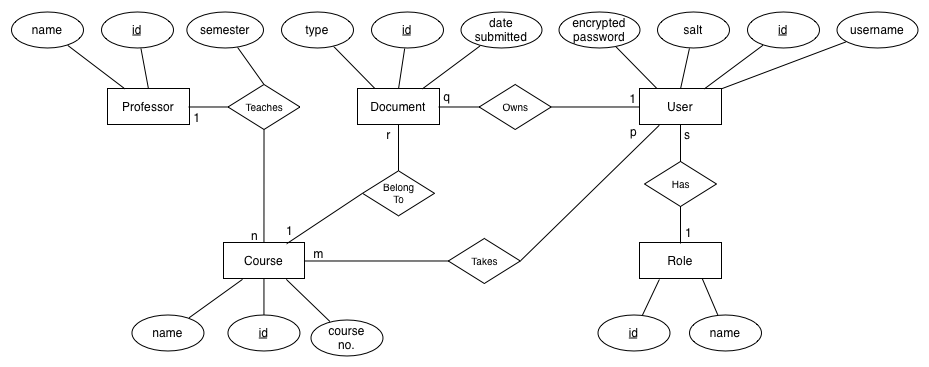
\includegraphics[width=.9\linewidth]{ER Diagram.png}

\end{document}